\section{Repetition/Introduction to Simulink/QuaRC}\label{sec:prob1}

\begin{table}[tbp]
	\centering
	\caption{Parameters and values.}
	\begin{tabular}{llll}
		\hline
		Symbol & Parameter & Value & Unit \\
		\hline
		$l_a$ & Distance from elevation axis to helicopter body & $0.63$ & \meter \\
		$l_h$ & Distance from pitch axis to motor & $0.18$ & \meter \\
		$K_f$ & Force constant motor & $0.25$ & \newton\per\volt \\
		$J_e$ & Moment of inertia for elevation & $0.83$ & \kilogram\usk\square\meter \\
		$J_t$ & Moment of inertia for travel & $0.83$ & \kilogram\usk\square\meter \\
		$J_p$ & Moment of inertia for pitch & $0.034$ & \kilogram\usk\square\meter \\
		$m_h$ & Mass of helicopter & $1.05$ & \kilogram \\
		$m_w$ & Balance weight & $1.87$ & \kilogram \\
		$m_g$ & Effective mass of the helicopter & $0.05$ & \kilogram \\
		$K_p$ & Force to lift the helicopter from the ground & $0.49$ & \newton \\
		\hline
	\end{tabular}
	\label{tab:parameters}
\end{table}
\subsection{PID-(re)tuning}

\subsection{Results and discussion}

\begin{figure}[hp]
	\centering
		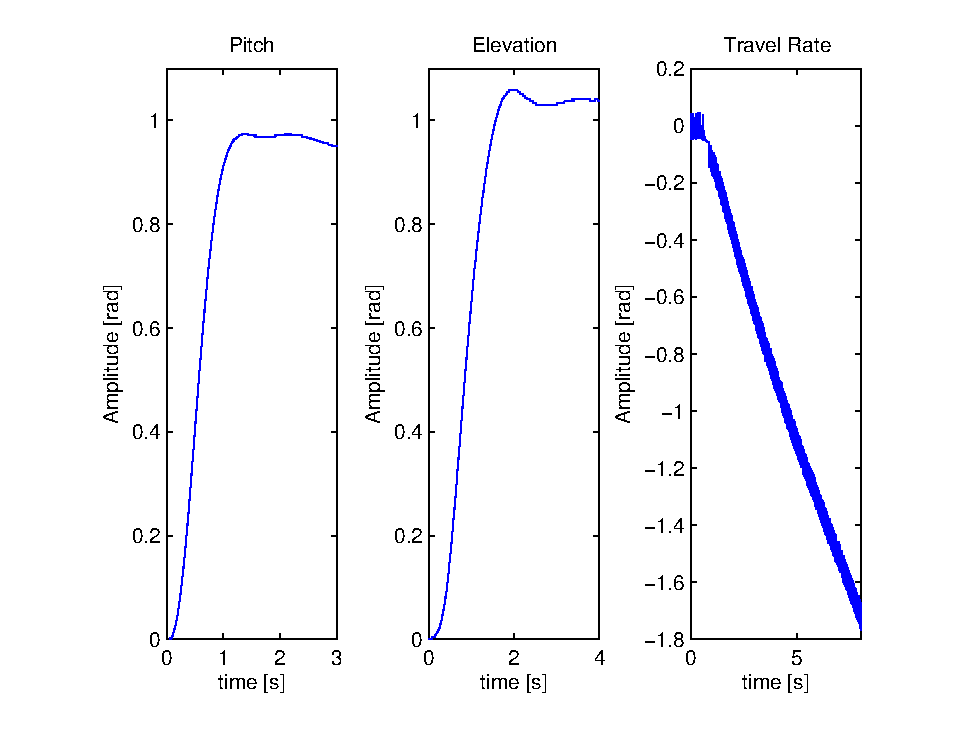
\includegraphics[width=1.00\textwidth]{figures/1/step_response.eps}
	\caption{Step response.}
	\label{fig:step_response}
\end{figure}

